%%%%%%%%%%%%%%%%%%%%%%%%%%%%%%%%%%%%%%%%%
% Stylish Article
% LaTeX Template
% Version 2.2 (2020-10-22)
%
% This template has been downloaded from:
% http://www.LaTeXTemplates.com
%
% Original author:
% Mathias Legrand (legrand.mathias@gmail.com) 
% With extensive modifications by:
% Vel (vel@latextemplates.com)
%
% License:
% CC BY-NC-SA 3.0 (http://creativecommons.org/licenses/by-nc-sa/3.0/)
%
%%%%%%%%%%%%%%%%%%%%%%%%%%%%%%%%%%%%%%%%%

%----------------------------------------------------------------------------------------
%	PACKAGES AND OTHER DOCUMENT CONFIGURATIONS
%----------------------------------------------------------------------------------------

\documentclass[fleqn,10pt]{SelfArx} % Document font size and equations flushed left

\usepackage[english]{babel} % Specify a different language here - english by default

\usepackage{lipsum} % Required to insert dummy text. To be removed otherwise

%----------------------------------------------------------------------------------------
%	COLUMNS
%----------------------------------------------------------------------------------------

\setlength{\columnsep}{0.55cm} % Distance between the two columns of text
\setlength{\fboxrule}{0.75pt} % Width of the border around the abstract

%----------------------------------------------------------------------------------------
%	COLORS
%----------------------------------------------------------------------------------------

\definecolor{color1}{RGB}{0,0,90} % Color of the article title and sections
\definecolor{color2}{RGB}{0,20,20} % Color of the boxes behind the abstract and headings

%----------------------------------------------------------------------------------------
%	HYPERLINKS
%----------------------------------------------------------------------------------------

\usepackage{hyperref} % Required for hyperlinks

\hypersetup{
	hidelinks,
	colorlinks,
	breaklinks=true,
	urlcolor=color2,
	citecolor=color1,
	linkcolor=color1,
	bookmarksopen=false,
	pdftitle={Title},
	pdfauthor={Author},
}

%----------------------------------------------------------------------------------------
%	ARTICLE INFORMATION
%----------------------------------------------------------------------------------------

\JournalInfo{Journal, Vol. XXI, No. 1, 1-5, 2013} % Journal information
\Archive{Additional note} % Additional notes (e.g. copyright, DOI, review/research article)

\PaperTitle{Crypto-currency ..} % Article title

\Authors{Shahmari Y.\textsuperscript{a}*, Yousefi Karkhane M.\textsuperscript{a}, Najafi K.\textsuperscript{a}, Jafari G.R.\textsuperscript{b}, Rouhani S.\textsuperscript{a}} % Authors
\affiliation{\textsuperscript{a}\textit{Department of Physics, Sharif University of Technology, Tehran, Iran}} % Author affiliation
\affiliation{\textsuperscript{b}\textit{Department of Physics, Shahhid Behesti University, Tehran, Iran}} % Author affiliation
\affiliation{*\textbf{Corresponding author}: y.shahmari@sharif.com} % Corresponding author

\Keywords{Blockchain -- Cryptocurrency -- Causality -- Granger test} % Keywords - if you don't want any simply remove all the text between the curly brackets
\newcommand{\keywordname}{Keywords} % Defines the keywords heading name

%----------------------------------------------------------------------------------------
%	My own Configurations
%----------------------------------------------------------------------------------------

\usepackage[section]{placeins}
\usepackage{graphicx, wrapfig, amsmath, amssymb, physics}
\graphicspath{ {../Figs/} }

%----------------------------------------------------------------------------------------
%	ABSTRACT
%----------------------------------------------------------------------------------------

\Abstract{The main question of this article is what are the interdependencies of crypto-currencies also of dependence on fiat currencies.  To answer this question we plot the minimal spanning tree of five crypto-currencies and five crypto plus ten fiat currencies. For this purpose we ..}

%----------------------------------------------------------------------------------------

\begin{document}
\maketitle % Output the title and abstract box

\tableofcontents % Output the contents section

\thispagestyle{empty} % Removes page numbering from the first page

%----------------------------------------------------------------------------------------
%	ARTICLE CONTENTS
%----------------------------------------------------------------------------------------

\section*{Introduction} % The \section*{} command stops section numbering

\addcontentsline{toc}{section}{Introduction} % Adds this section to the table of contents

The emergence of blockchain technology and cryptocurrencies has received significant attention in recent years. The original cryptocurrency, named Bitcoin was introduced as a proof of concept by an unknown author or authors (Nakamoto, 2009). Bitcoin was originally designed as a proof of concept for a trustless medium of exchange (Dyhrberg, 2016). However, cryptocurrencies proliferated and were used as investment assets. Many studies have focused on the investment asset nature of cryptocurrencies (Baur, 2018). However, Cryptocurrency presents serious challenges to a government authority (European Central Bank, 2012). Economies have become dependent on cryptocurrency (Alireza Manaviab, 2020) Also political upheaval will reflect in crypto fluctuations, which we will demonstrate here. We have tried to look at a number of questions raised by crypto currencies….

%------------------------------------------------

\section{Materials and Methods}

We have used commonly used functions and methods in time series analysis, which we briefly discuss here. 

\subsection{Data preparation and structure}

*Shahmari*

\subsection{Mathematical Methods}

\subsubsection{Correlation}

The correlation between two time series X1 and X2 is defined as:

\begin{equation}
	\mathrm{Corr}(X_1, X_2) = \frac{\mathrm{Cov}(X_1, X_2)}{\sqrt{\mathrm{Var}(X_1)\mathrm{Var}(X_2)}} = \frac{(x-\langle x\rangle)(y-\langle y\rangle)}{\|x-\langle x\rangle\|\|y-\langle y\rangle\|}
	\label{eq:refname2}
\end{equation}

\subsubsection{Granger Test}

\subsubsection{Eddy-Fuller Test}

\subsubsection{Minimal Spanning Tree}

*Karkhaneh-Yousefi*

\subsubsection{Volatility study}

*Shahmari*

\subsubsection{Macroscopic time dependence}

\paragraph{Correlation with fiat currencies}

We calculate and plot the correlation Eq.(1)  of BTC prices for various fiat currencies. Clearly such correlation is calculated over a span of time which is taken as 60 days. However, the center of this window is moved over two years. We observe a marked fall in Ruble, which is coincident with Ukraine war. Curiously the correlation picks up again after a while and is in line with other currencies. 

\begin{figure}[!htb]
	\centering
	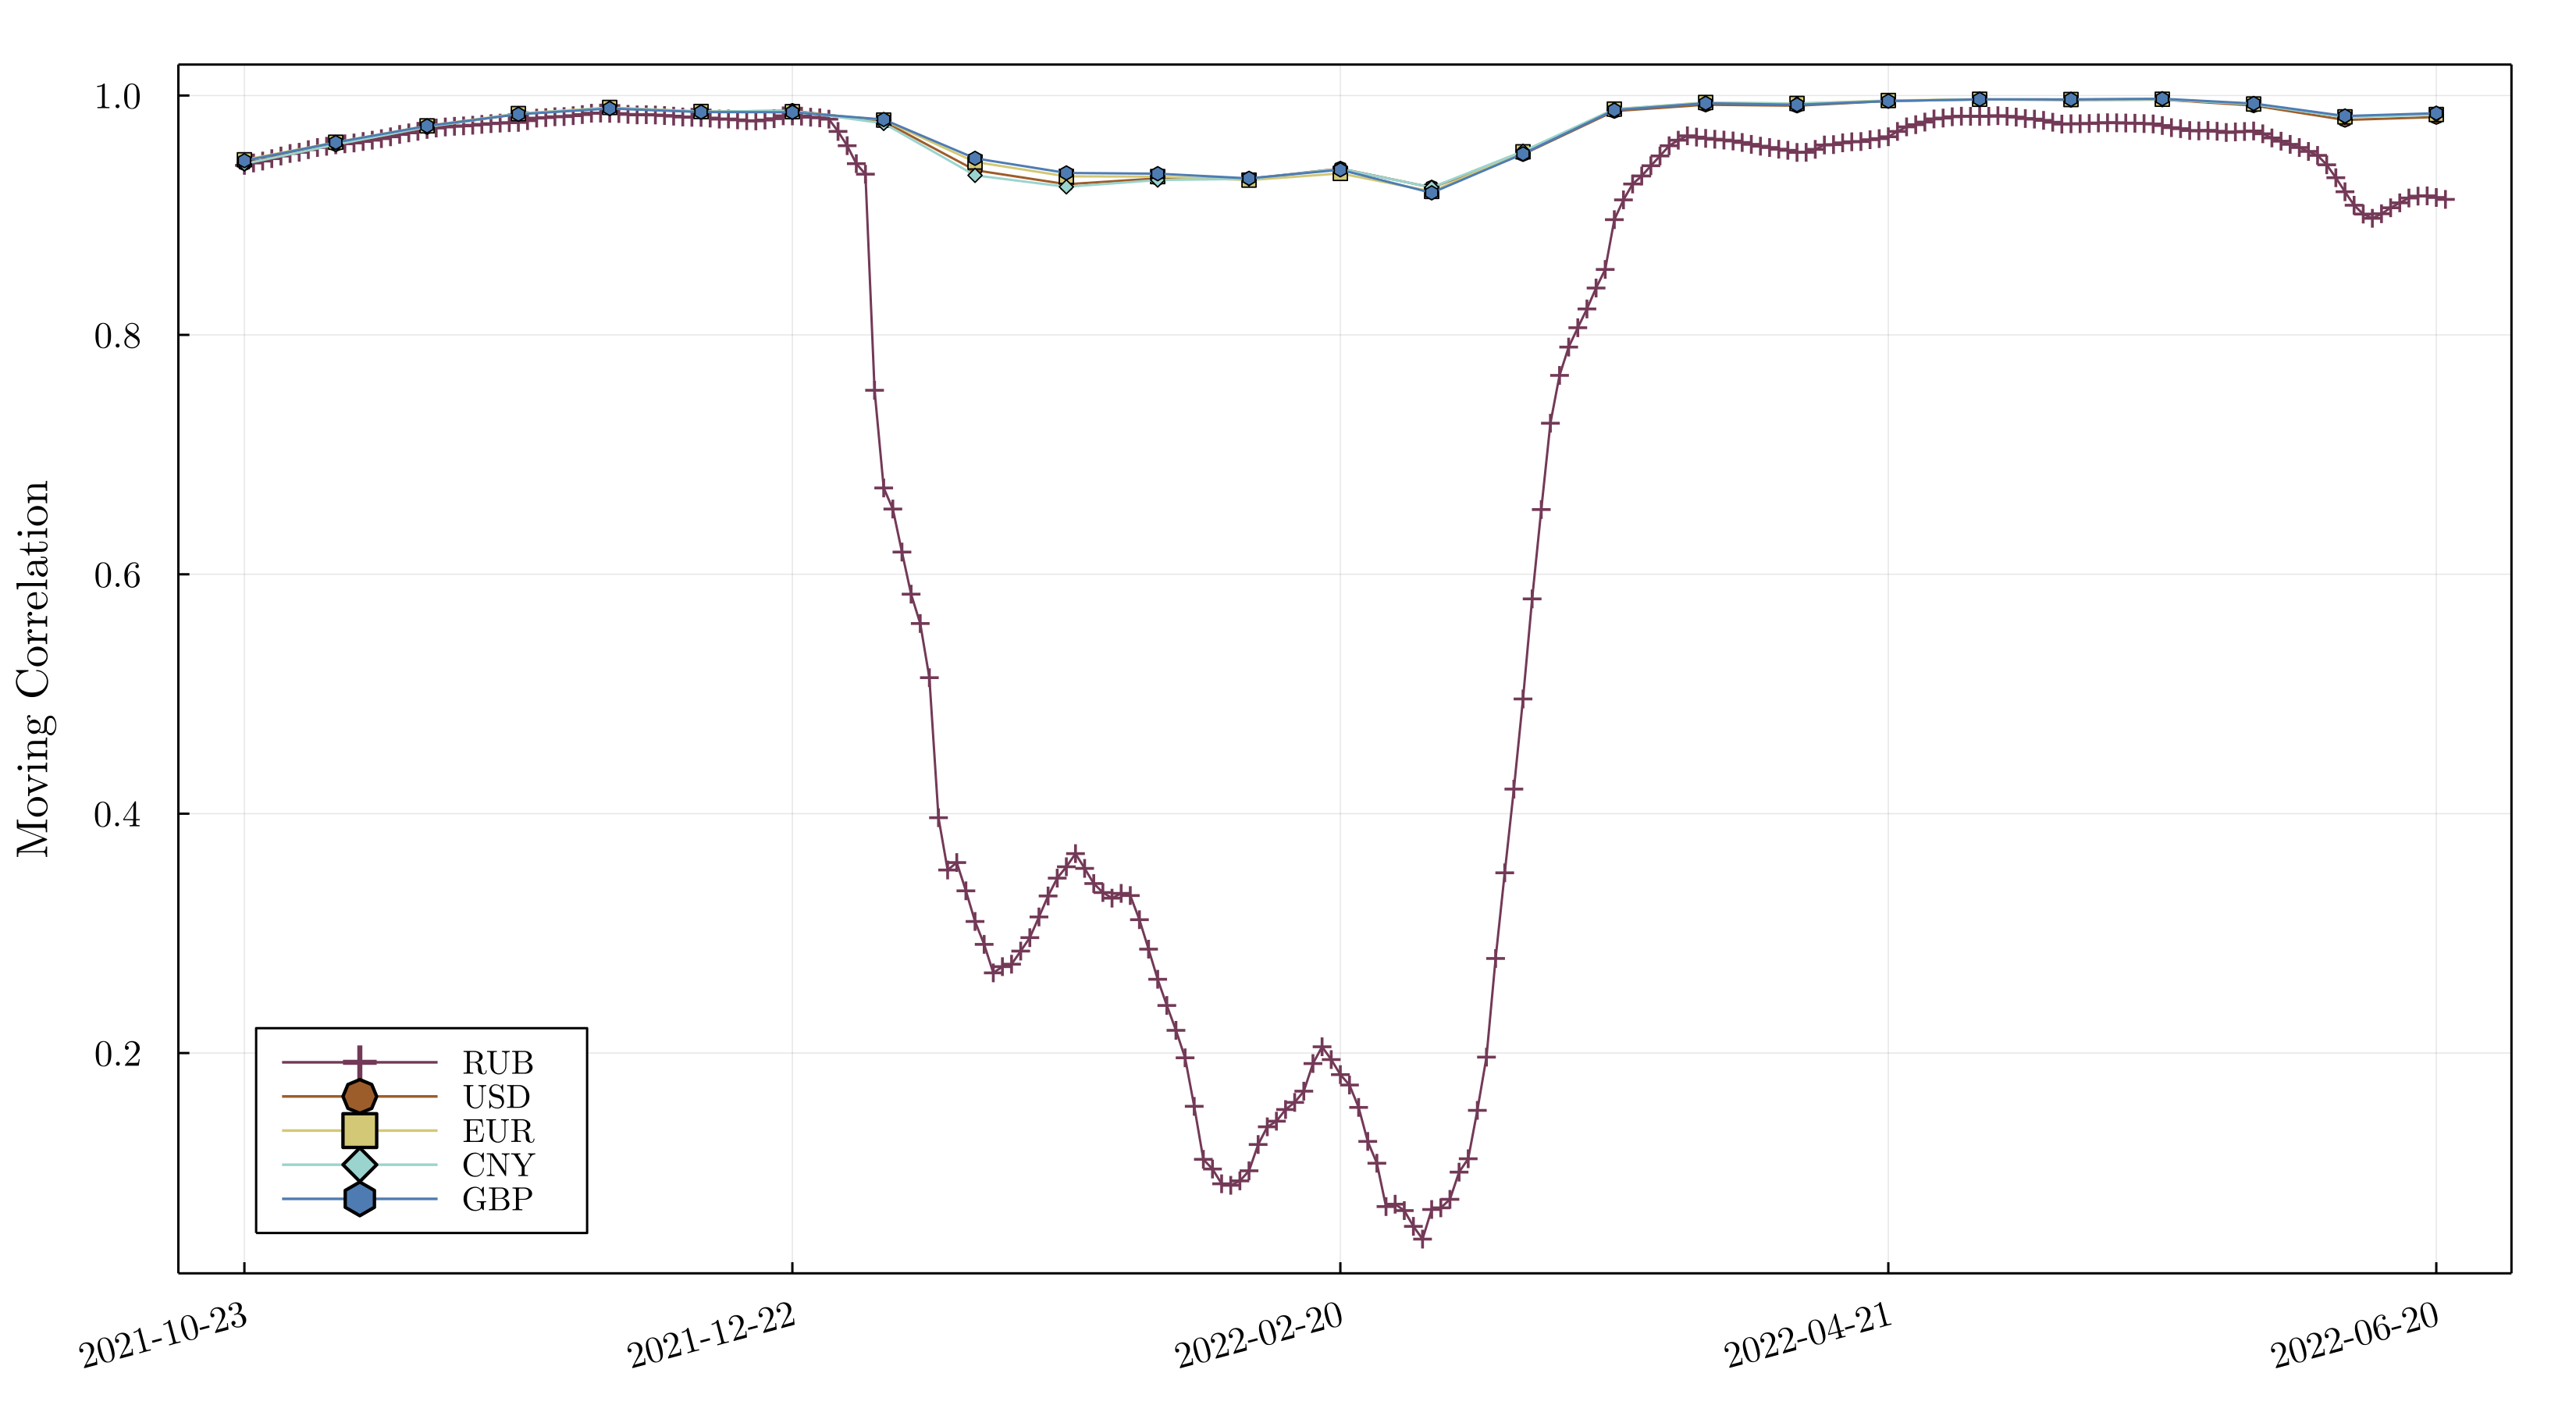
\includegraphics[scale = 0.2]{/MovingCorrelation-BTCPrice-FinnoRussoWar}
	\label{fig.1}
	\caption{Moving correlation of BTC prices with some fiat currencies.}
\end{figure}

Plotting the correlation Eq.(1)  of BTC prices for a larger family of fiat currencies and over much longer window i.e. 7 years results in the graph of Fig. 2. We observe that some fiat currencies show a marked fluctuation. Some currencies show sudden and sharp fall such as Nigeria and Turkey. These peaks seem to show a width of several months. May have to do with some economic decisions in these countries.
Furthermore we observe a sharp fall in NGN , which is associated with a fluctuation in GBP and UAH. Towrds the end of the graph we also see sharp falls in RUB and UAH too.

\begin{figure}[!htb]
	\centering
	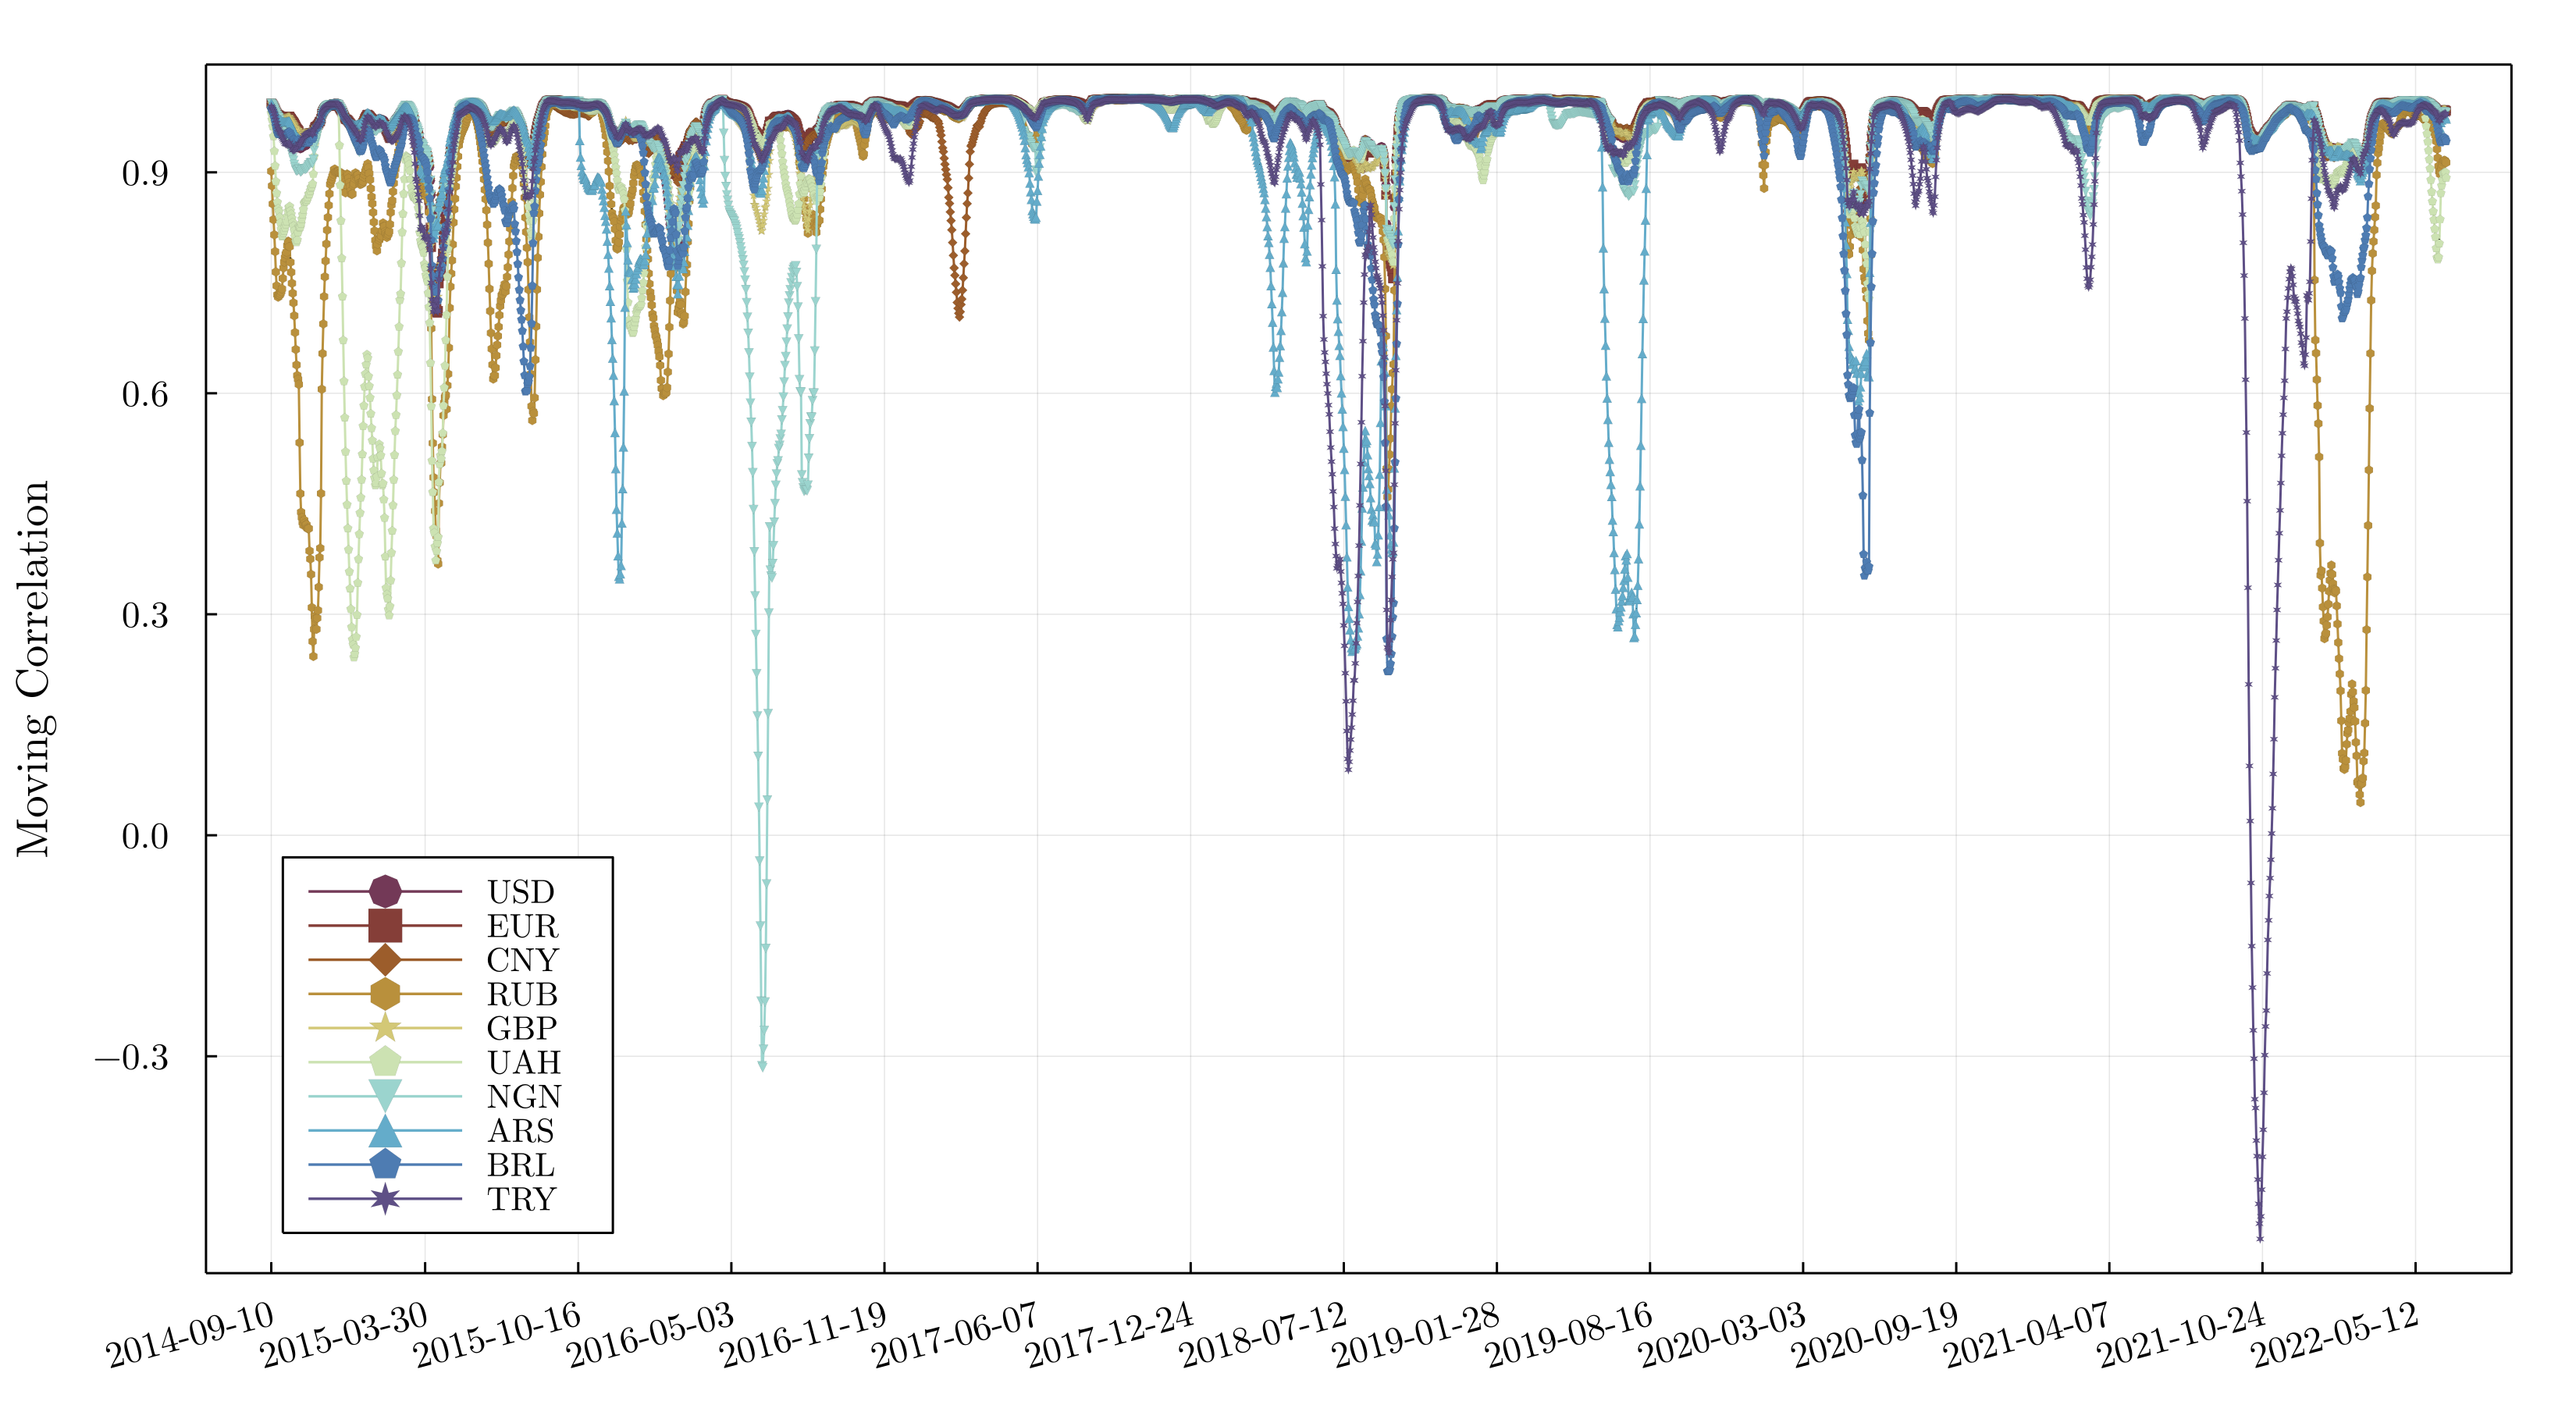
\includegraphics[scale = 0.0675]{/MovingCorrelation-BTCPrice-Overview.png}
	\label{fig.2}
	\caption{Moving correlations for BTC versus some fiat currencies over a much longer (seven-year) period.}
\end{figure}

Looking at volumes of trade instead of price, a similar picture emerges.

\begin{figure}[!htb]
	\centering
	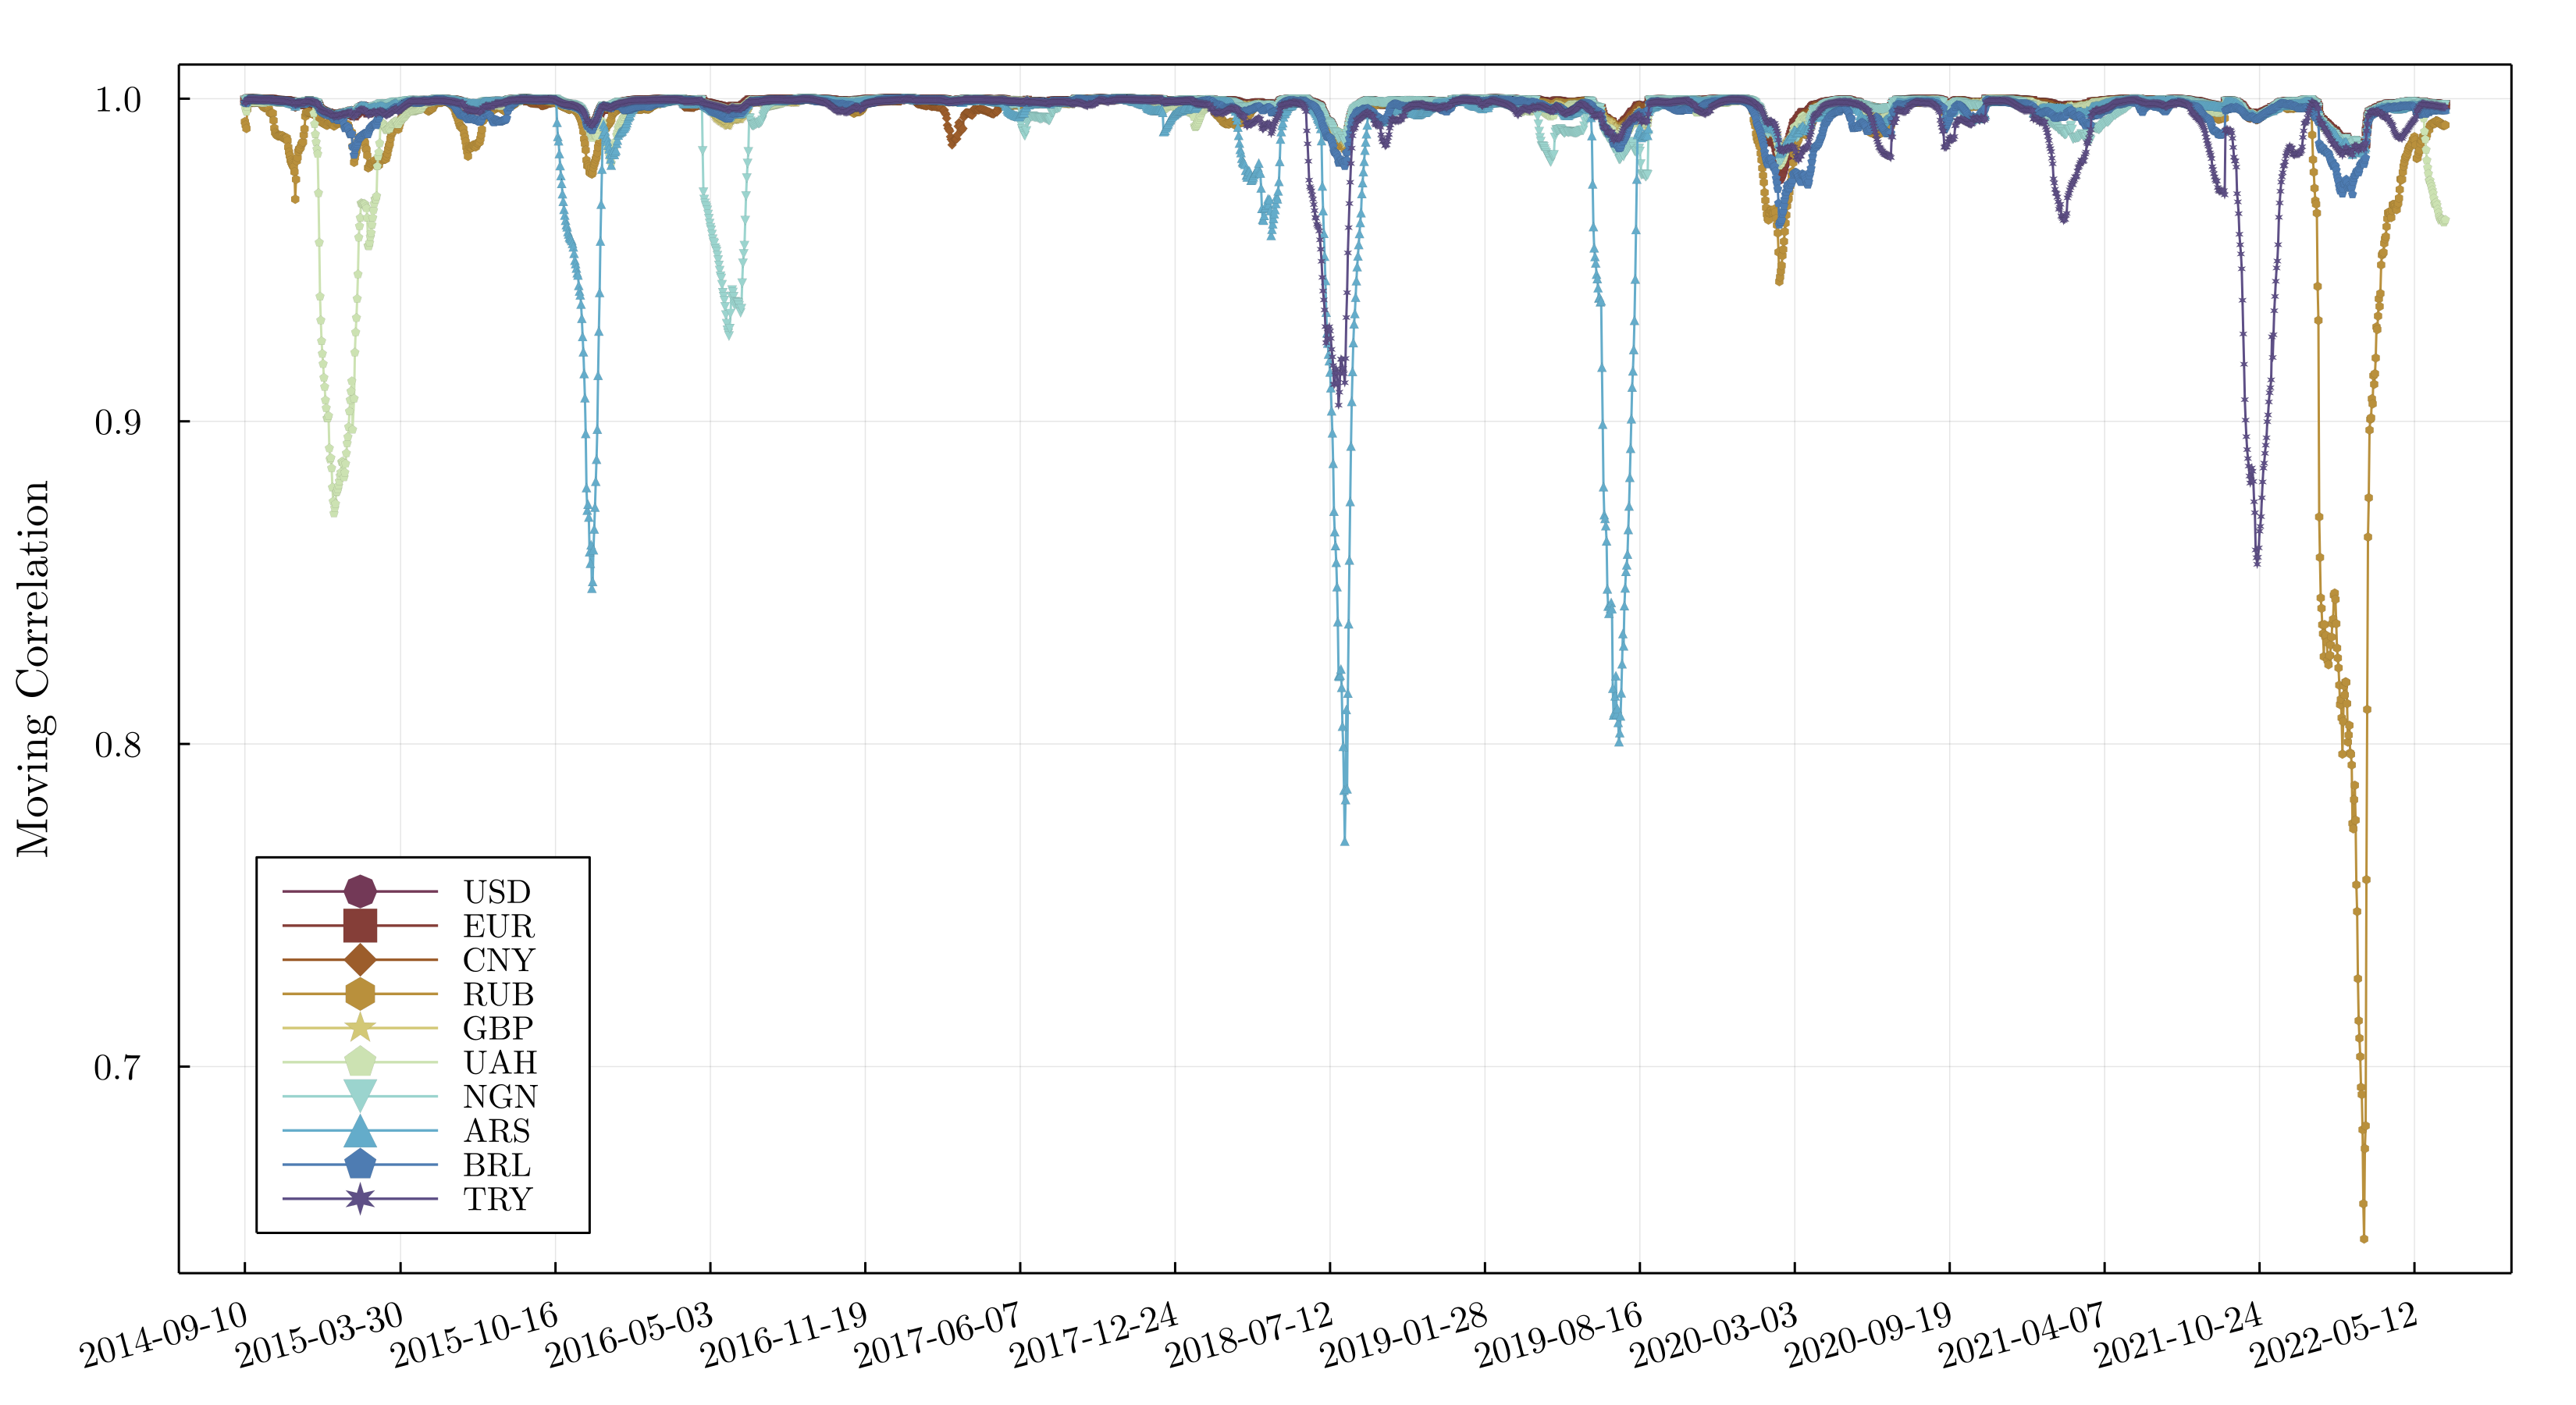
\includegraphics[scale = 0.0675]{/MovingCorrelation-BTCVolume-Overview.png}
	\label{fig.3}
	\caption{Fluctuations in volume of BTC sold over some fiat currencies.}
\end{figure}

\section{Results and discussion}

\subsection{Minimal Spanning Tree}

A minimum spanning tree (MST) is a graph that connects all the vertices together, with the minimum possible total edge weight. [1] That is, it is a spanning tree whose sum of edge weights is as small as possible. For this purpose, we calculate the matrix of F and P values from the granger test. Below the P-values matrix for a number of cryptos is given. 

%------------------------------------------------

\phantomsection
\section*{Acknowledgments} % The \section*{} command stops section numbering

\addcontentsline{toc}{section}{Acknowledgments} % Adds this section to the table of contents

So long and thanks for all the fish \cite{Figueredo:2009dg, Smith:2012qr}.

%----------------------------------------------------------------------------------------
%	REFERENCE LIST
%----------------------------------------------------------------------------------------

\phantomsection
\bibliographystyle{unsrt}
\bibliography{bibliography.bib}

%----------------------------------------------------------------------------------------

\end{document}